\documentclass[a4paper,14pt]{extreport} % формат документа

\usepackage{amsmath}
\usepackage{cmap} % поиск в ПДФ
\usepackage[T2A]{fontenc} % кодировка
\usepackage[utf8]{inputenc} % кодировка исходного текста
\usepackage[english,russian]{babel} % локализация и переносы
\usepackage[left = 2cm, right = 1cm, top = 2cm, bottom = 2 cm]{geometry} % поля
\usepackage{listings}
\usepackage{graphicx} % для вставки рисунков
\usepackage{amsmath}
\usepackage{float}
\usepackage{multirow}
\graphicspath{{pictures/}}
\DeclareGraphicsExtensions{.pdf,.png,.jpg}
\newcommand{\anonsection}[1]{\section*{#1}\addcontentsline{toc}{section}{#1}}

\lstset{ %
	language=Lisp,                % Язык программирования 
	numbers=left,                   % С какой стороны нумеровать          
	frame=single,                    % Добавить рамку
}

\begin{document}
\begin{titlepage}

    \begin{table}[H]
        \centering
        \footnotesize
        \begin{tabular}{cc}
            \multirow{8}{*}{
\includegraphics[scale=0.35]{bmstu.jpg}}
            & \\
            & \\
            & \textbf{Министерство науки и высшего образования Российской Федерации} \\
            & \textbf{Федеральное государственное бюджетное образовательное учреждение} \\
            & \textbf{высшего образования} \\
            & \textbf{<<Московский государственный технический} \\
            & \textbf{университет имени Н.Э. Баумана>>} \\
            & \textbf{(МГТУ им. Н.Э. Баумана)} \\
        \end{tabular}
    \end{table}

    \vspace{-2.5cm}

    \begin{flushleft}
        \rule[-1cm]{\textwidth}{3pt}
        \rule{\textwidth}{1pt}
    \end{flushleft}

    \begin{flushleft}
        \small
        ФАКУЛЬТЕТ
        \underline{<<Информатика и системы управления>>\ \ \ \ \ \ \ 
        \ \ \ \ \ \ \ \ \ \ \ \ \ \ \ \ \ \ \ \ \ \ \ \ \ \ \ \ \ \ \ 
    \ \ \ \ \ \ \ \ \ \ \ \ \ \ \ } \\
        КАФЕДРА
        \underline{<<Программное обеспечение ЭВМ и
        информационные технологии>>
        \ \ \ \ \ \ \ \ \ \ \ \ \ \ \ \ \ \ \ \ }
    \end{flushleft}

    \vspace{2cm}

    \begin{center}
        \textbf{Лабораторная работа № 6} \\
        \vspace{0.5cm}
    \end{center}

    \vspace{4cm}

    \begin{flushleft}
        \begin{tabular}{ll}
            \textbf{Дисциплина} & Моделирование.  \\
            \textbf{Тема} & Кинотеатр.  \\
            \\
            \textbf{Студент} & Сиденко А.Г. \\
            \textbf{Группа} & ИУ7-73Б \\
            \textbf{Оценка (баллы)} & \\
            \textbf{Преподаватель} & Рудаков И.В.   \\
        \end{tabular}
    \end{flushleft}

    \vspace{4cm}

   \begin{center}
        Москва, 2020 г.
    \end{center}

\end{titlepage}

\begin{enumerate}

\item \textbf{Условие. }

В кинотеатр приходят посетители через интервал времени 10 $\pm$ 5 минут. По правилам соблюдения социальной дистанции, если в очереди на проверку наличия маски больше одного человека, посетителю отказывается в обслуживании. Время проверки маски -- 1 минута. Также с вероятностью 10\% посетитель будет без маски и ему будет отказано. Если два из имеющихся термометров заняты, клиенту отказывают в обслуживании. Время работы термометров 2 $\pm$ 1 минута, с вероятностью 5\% посетитель будет с температурой и ему будет отказано. Далее посетители проходят  в очередь на кассу для покупки билетов. Кассир обслуживает посетителей за 7 $\pm$ 5 минут, максимальная длина очереди 5 человек.  Далее посетители проходят за едой и напитками, однако если в каждой очереди более двух человек, они сразу проходят на проверку билетов.  В кассах еды и напитков, время обслуживания: первая -- 7 $\pm$ 5 минут, вторая -- 3 $\pm$ 2 минуты, третья -- 5 $\pm$ 2 минуты. После посетитель проходят в очередь на проверку билетов, проверка занимает 2 минуты. Промоделировать процесс полного заполнения зала на 100 человек. 

Найти вероятность отказа. 

\item \textbf{Теория. }

В соответствии с концептуальной схемой построим структурную схему, представленную на рисунке \ref{model}. 

\begin{figure}[H]
  \centering
  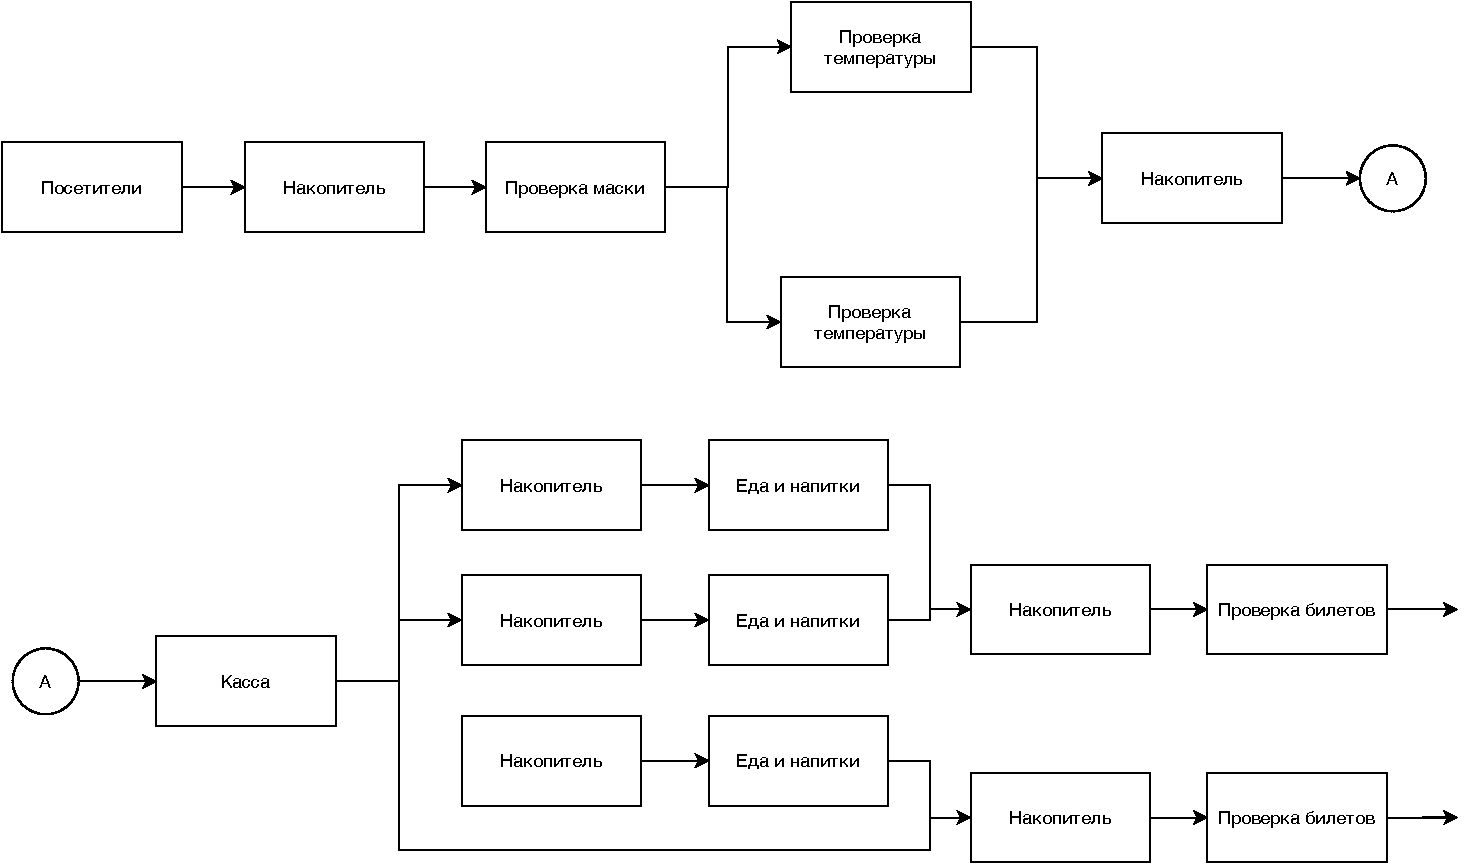
\includegraphics[scale=0.75]{model}
  \caption{Концептуальная схема.  }
  \label{model}
\end{figure}

Вероятность отказа -- это промежуток, для этого прогоним модель 10 раз и выберем максимальное и минимальное значение. 

\item \textbf{Полученные результаты. }

Ниже представлены результаты -- промежутки, в которых может находиться вероятность отказа и количество отказов. 

\begin{figure}[H]
  \centering
  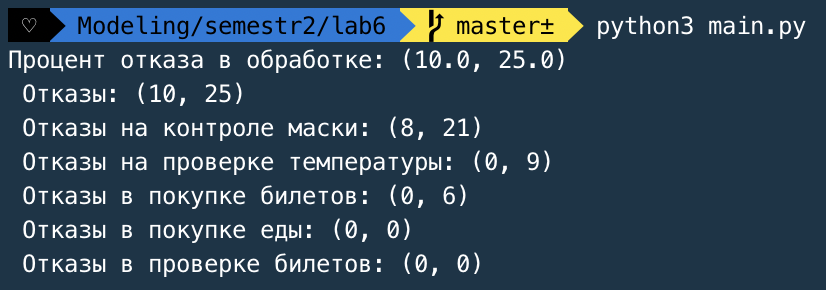
\includegraphics[scale=0.7]{1}
  \caption{Пример. }
\end{figure}

Как видим из результатов на этапе контроля маски и проверки температуры возникают отказы по причине не соблюдения правил (отсутствие маски и наличие температуры) и по причине ограничения длины очереди. Также может быть отказано на этапе покупки билетов, при превышении очереди в 5 человек. На этапе покупки еды, если очередь длинная, посетитель идет на проверку билетов, где также отказов быть не должно. 

\item \textbf{Вывод. }

Была смоделирована система кинотеатра, в которую приходят посетители. Данная система состоит из нескольких блоков: контроль маски, проверка температуры, билетные кассы, касса еды и напитков, проверка билетов и накопители. 

На выходе получаем число клиентов получивших отказ и вероятность отказа на каждом этапе и в общем. 

\end{enumerate}


\end{document}